%Fiquemos com Deus e Nossa Senhora!
%Sao Jose de Cupertino rogai por nos!!
% ### Uses XeLaTeX ### %
% ### Needs beamer-master ### %
\documentclass[aspectratio=169]{beamer} %. Aspect Ratio 16:9

\usetheme{AI2} % beamerthemeSprace.sty
\usepackage[portuguese]{babel}
\usepackage[utf8]{inputenc}
\usepackage[T1]{fontenc}
\usepackage{ragged2e,gensymb}

\DeclareMathOperator*{\argmin}{arg\,min}
\DeclareMathOperator*{\argmax}{arg\,max}
\DeclareMathOperator{\sign}{sgn}

% DATA FOR FOOTER
\date{2021}
\title{- Classificador Bayesiano}
\author{João Paulo Papa}
\institute{Advanced Institute for Artificial Intelligence (AI2)}

\begin{document}
% ####################################
% FIRST SLIDE 						:: \SliTit{This is the Title of the Talk}{A. B. Name}{Sprace}
% SUB-TITLE SLIDE 					:: \SliSubTit{<title>}{<explanation}
% SUB-SUB-TITLE SLIDE				:: \SliSubSubTit{<title>}{<explanation}
% SLIDE WITH TITLE 					:: \SliT{Title}{Content}
% SLIDE NO TITLE 						:: \Sli{Content} 
% SLIDE DOUBLE COLUMN WITH TITLE 	:: \SliDT{Title}{First Column}{Second Column}
% SLIDE DOUBLE COLUMN NO TITLE 		:: \SliD{First Column}{Second Column}
% SLIDE ADVANCED WITH TITLE 			:: \SliAdvT{Title}{Content}
% SLIDE ADVANCED NO TITLE 			:: \SliAdv{Content}
% SLIDE ADVANCED DOUBLE WITH TITLE 	:: \SliAdvDT{Title}{First Column}{Second Column}
% SLIDE ADVANCED DOUBLE NO TITLE 	:: \SliAdvD{First Column}{Second Column}
% SLIDE BLACK						:: \Black{ <Content> }
% SLIDE WHITE						:: \White{ <Content> }
% ITEMIZATION 						:: \begin{itemize}  \iOn{First} \iTw {Second} \iTh{Third} \end{itemize}
% COMMENT TEXT				 		:: \note{<comment>}
% SECTION 							:: \secx{Section} | \secxx{Sub-Section}
% BOLD SPRACE COLOR				:: \bfs{<text>}
% TABLE OF CONTENT					:: \tocitem{<title>}{<content>}
% LEFT ALIGN EQUATION				:: \begin{flalign*}  & <equation> &   \end{flalign*}
% CENTER ALIGN EQUATION	S			:: \begin{gather*} <equations>  \end{gather*}
% SLASH								:: \slashed{<>}
% BAR								:: \barr{<letter>} instead of \bar{<letter>}
% THEREFORE						:: use \portanto (larger and bold}
% 2 or 3 MATH SYMBOLS				:: \overset{<up>}{<down>} &  \underset{<below>}{\overset{<above>}{<middle>}}  
% INSERT TEXT IN FORMULA			:: \ins{<text>}
% EXERCISE							:: \exe{<exercise #>}{<exercise text>}
% SUGGESTED READING BOX			:: \sug{<references>}
% CITATION							:: \cittex{<citation>}
% CITATION DOUBLE COLUMN 			:: \cittexD{<citation>}
% TEXT POSITION						:: \texpos{<Xcm>}{<Ycm>}{<text>} origin = center of slide : x right | y down
% REFERENCE AT BOTTOM  S/D SLIDE		:: \refbotS{<reference>} \refbotD{<reference>}
% HIDDEN SLIDE						:: \hid
% COLOR BOX 						:: \blu{blue} + \red{rec} + \yel{yellow} + \gre{green} + \bege{beige}
% FRAME 							:: \fra{sprace} \frab{blue} \frar{red} + \fray{yellow} + \frag{green}		
% FIGURE 							:: \img{X}{Y}{<scale>}{Figure.png} 
% FIGURE							:: \includegraphics[scale=<scale>]{Figures/.png}
% FIGURE DOUBLE SLIDE NO TITLE		::  \img{-4}{0.5}{<scale>}{Figure.png} % Image 1st half
%									::  \img{4}{0.5}{<scale>}{Figure.png} % Image 2nd half
% FIGURE DOUBLE SLIDE WITH TITLE		::  \img{-4}{0}{<scale>}{Figure.png} % Image 1st half
%									::  \img{4}{0}{<scale>}{Figure.png} % Image 2nd half
% INCLUDING SWF (Flash)				:: \usepackage{media9} and \includemedia >> USE ACROBAT <<
%%%%%%%%%%%%%%%%%%%%%%%%%%%%%%%%%%%%%%%%%%%%%%%%%%
% ###############################################################################
% FIRST SLIDE
\SliTit{{\LARGE Classificador Bayesiano}}{Advanced Institute for Artificial Intelligence -- AI2}{https://advancedinstitute.ai}
%%%%%%%%%%%%%%%%%%%%%%%%%%%%%%%%%%%%%%%%%%%%%%%%%%
% ###############################################################################
% SLIDE SUB-TITLE
%\SliSubTit{Sub-Title}{Description}{}
%%%%%%%%%%%%%%%%%%%%%%%%%%%%%%%%%%%%%%%%%%%%%%%%%%
% ###############################################################################
%\SliSubSubTit{Sub-Sub-Title}{Description}
 %%%%%%%%%%%%%%%%%%%%%%%%%%%%%%%%%%%%%%%%%%%%%%%%%%


\SliT{Introdução}{

\justifying A Teoria de Decisão Bayesiana é um ferramental matemático que nos permite construir classificadores \textbf{paramétricos}, ou seja, técnicas que assumem a hipótese de que os dados seguem alguma distribuição (hipótese Gaussiana na grande maioria dos casos).\newline

\justifying \underline{Definição do problema:} seja ${\cal X}^1=\{(\boldsymbol{x}_1,y_1),(\boldsymbol{x}_2,y_2),\ldots,(\boldsymbol{x}_m,y_m)\}$ um conjunto de dados de treinamento tal que $\boldsymbol{x}_i\in\mathbb{R}^n$ corresponde a uma amostra e $y_i\in{\cal Y}$ representa o rótulo dessa amostra, em que ${\cal Y}=\{\omega_1,\omega_2,\ldots,\omega_c\}$.
}

\Sli{
Além disso, temos os seguintes componentes em nosso ferramental:

\begin{itemize}
	\item $p(\omega_i)$: \textbf{probabilidade a priori} da classe $\omega_i$ (proporção). Ex: em um problema de classificar indivíduos em jogadores de futebol ($\omega_1$) ou basquete ($\omega_2$), se nós temos $90$ jogadores de futebol e $10$ de basquete, então $p(\omega_1) = 0.9$ e $p(\omega_2) = 0.1$. Na prática, $p(\omega_1)$ denota a probabilidade de, ao selecionar algum jogador de maneira aleatória, ele ser um jogador de futebol. O mesmo vale para $p(\omega_2)$.
\end{itemize}
}

\Sli{
\begin{itemize}
	\item $p(\boldsymbol{x}|\omega_i)$: \textbf{probabilidade condicional} da classe $\omega_i$ (verossimilhança). Ela descreve a função de densidade de probabilidade, ou seja, qual o comportamento de $\boldsymbol{x}$ dentro da classe $\omega_i$. Ex: se $\boldsymbol{x}$ corresponde à altura do jogador em metros, $p(\boldsymbol{x}|\omega_i)$ descreve a distribuição das alturas dos jogadores de futebol e $p(\boldsymbol{x}|\omega_2)$ descreve a distribuição das alturas dos jogadores de basquete. Assumindo que temos uma hipótese Gaussiana, podemos representar $p(\boldsymbol{x}|\omega_i)$ como segue:
\end{itemize}
\vspace{-0.1cm}
\begin{minipage}{0.49\textwidth}
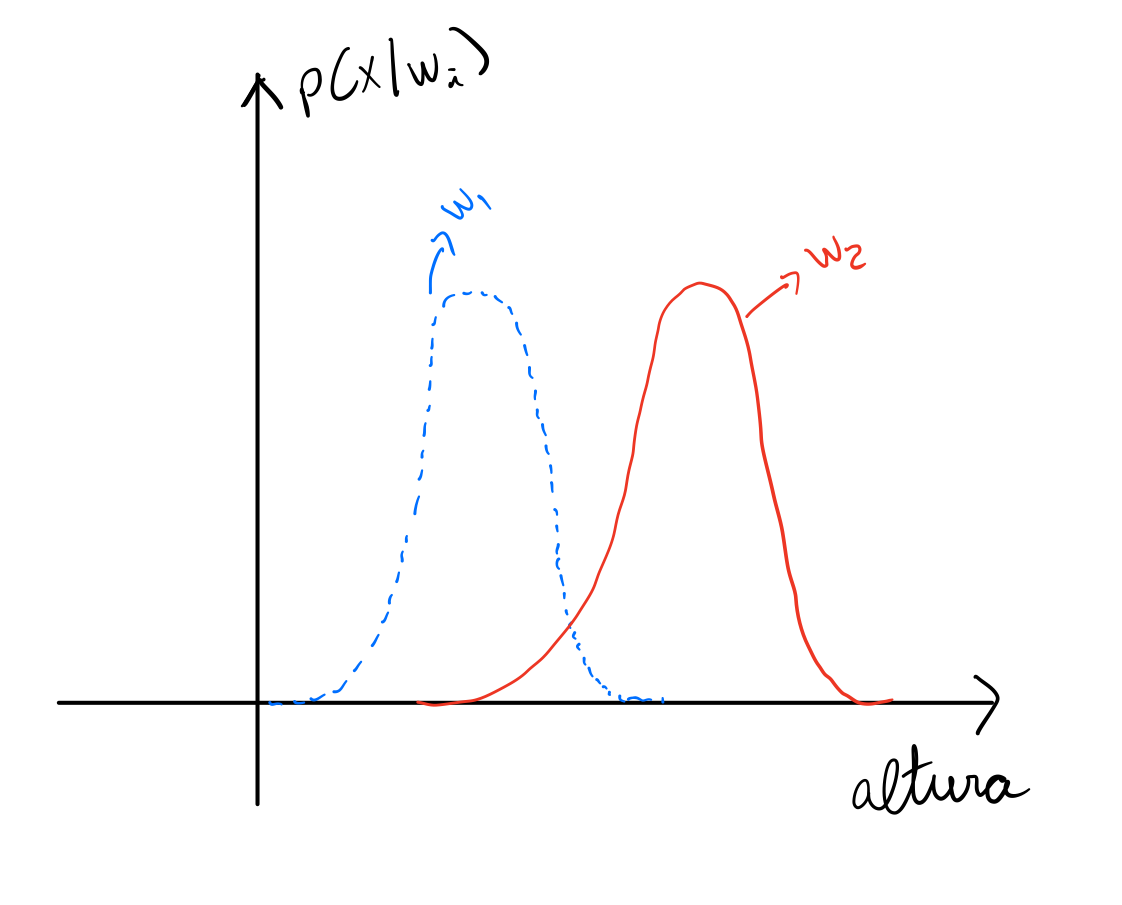
\includegraphics[scale=0.15]{./figs/Bayes_Fig1.png}
\end{minipage}%%% to prevent a space
\begin{minipage}{0.37\textwidth}
$p(\boldsymbol{x}|\omega_1)\sim{\cal N}(\mu_1,\sigma^2_1)$\\
$p(\boldsymbol{x}|\omega_2)\sim{\cal N}(\mu_2,\sigma^2_2)$
\null
\par\xdef\tpd{\the\prevdepth}
\end{minipage}
}

\Sli{
\begin{itemize}
\item $p(\omega_i|\boldsymbol{x})$: \textbf{probabilidade a posteriori} da classe $\omega_i$, isto é, a probabilidade de decidirmos pela classe $\omega_i$ dada que observamos a amostra $\boldsymbol{x}$.
\end{itemize}

Dados esses três componentes, temos que a regra de Bayes é formulada como segue:

\begin{equation}
	p(\omega_i|\boldsymbol{x}) = \frac{p(\boldsymbol{x}|\omega_i)p(\omega_i)}{p(\boldsymbol{x})},
\end{equation}
em que $p(\boldsymbol{x})$ é uma constante normalizadora que não depende da classe, calculada como segue:

\begin{equation}
	p(\boldsymbol{x}) = \sum_{j=1}^cp(\boldsymbol{x}|\omega_j)p(\omega_j).
\end{equation}
A fórmula acima faz com que $p(\omega_i|\boldsymbol{x})\in[0,1]$.
}

\SliT{Classificador Bayesiano sob Hipótese Gaussiana}{
\secx{Caso Unidimensional}

\justifying Neste caso, temos que nossa amostra $x\in\mathbb{R}$, ou seja, temos apenas uma única característica. Como em nosso exemplo anterior de classificar um jogador como sendo de basquete ou futebol, assuma que $x$ seja dado pela altura dos indivíduos.\newline

\justifying No caso unidimensional, temos que a probabilidade condicional da classe $\omega_i$ é dada por:

\begin{equation}
	p(x|\omega_i) = \frac{1}{\sqrt{2\pi\sigma^2_i}}\exp\left\{\frac{-(x-\mu_i)^2}{2\sigma^2_i}\right\}.
\end{equation}
}

\Sli{
\justifying A equação de uma função de densidade probabilidade Gaussiana possui dois parâmetros, isto é, a média $\mu_i$ e a variância $\sigma^2_i$, $\forall i=1,2,\ldots,c$. Assim sendo, a etapa de treinamento do classificador Bayesiano consiste em estimar esses parâmetros a partir dos dados de treinamento. Dado um problema com $c$ classes, o objetivo é aprender esses parâmetros para cada Gaussiana, isto é, uma para cada classe. Denotamos por $\boldsymbol{\theta}=\{\theta_1,\theta_2,\ldots,\theta_c\}$ esse conjunto de parâmetros a ser aprendido, em que $\theta_i = (\mu_i,\sigma^2_i)$.\newline

\justifying Um dos métodos mais conhecidos para aprendizado do conjunto de parâmetros $\boldsymbol{\theta}$ é o da máxima verossimilhança, ou seja, queremos maximizar a verossimilhança sobre o conjunto de dados de treinamento. Seja ${\cal X}^1_i\subset{\cal X}^1$ o subconjunto dos dados de treinamento que contém apenas amostras da classe $\omega_i$, $\forall i=1,2,\ldots,c$. Desta forma, o método da máxima verossimilhança consiste em encontrar $\theta_i$ que satisfaz a seguinte formulação:

\begin{equation}
	\hat{\mu_i},\hat{\sigma}^2_i = \argmax_{\mu_i,\sigma^2_i}\{p({\cal X}^1_i;\theta_i)\}.
\end{equation}
}

\Sli{
\justifying Temos que $p({\cal X}^1_i;\theta_i)$ corresponde à \textbf{densidade conjunta} das amostras da classe $\omega_i$ em função dos parâmetros:

\begin{equation}
	p({\cal X}^1_i;\theta_i) = \prod_{x_j\in{\cal X}^1_i}p(x_j;\theta_i),
\end{equation}
em que $p(x_j;\theta_i)=\frac{1}{\sqrt{2\pi\sigma^2_i}}\exp\left\{\frac{(x_j-\mu_i)^2}{2\sigma^2_i}\right\}$ possui a mesma formulação da Equação 3.
}

\Sli{
\justifying Para fins de tratabilidade matemática, é comum maximizar o logaritmo da verossimilhança, ou seja:

\begin{equation}
	\log p({\cal X}^1_i;\theta_i)=\sum_{x_j\in{\cal X}^1_i}\log p(x_j;\theta_i).
\end{equation}
A equação acima, após algumas derivações matemáticas, resulta em:

\begin{equation}
	\log p({\cal X}^1_i;\theta_i)=-\frac{m_i^\prime}{2}\log2\pi-\frac{m_i^\prime}{2}\log\sigma^2_i-\frac{1}{2\sigma^2_i}\sum_{x_j\in{\cal X}^1_i}(x_j-\mu_i)^2,
\end{equation}
em que $m_i^\prime = |{\cal X}^1_i|$.
}

\Sli{
\justifying Assim sendo, nosso problema passar a ser encontrar o conjunto de parâmetros $\theta_i$ que maximiza a seguinte equação:

\begin{equation}
\hat{\mu}_i,\hat{\sigma}_i = \argmax_{\mu_i\sigma_i^2}\{\log p({\cal X}^1_i;\theta_i)\}.
\end{equation}
Note que essa formulação precisa ser realizada para todas as classes, ou seja, $i=1,2,\ldots,c$.\newline

\justifying Para resolvermos o problema acima, basta calcular a derivada de $\log p({\cal X}^1_i;\theta_i)$ em relação à cada um dos seus parâmetros e igualar à zero, ou seja:

\begin{equation}\nonumber
	\frac{\partial \log p({\cal X}^1_i;\theta_i)}{\partial\mu_i}\text{\ \ e\ \ }\frac{\partial \log p({\cal X}^1_i;\theta_i)}{\partial\sigma_i^2}.
\end{equation}
}

\Sli{
Vamos calcular a derivada da função em relação ao parâmetro $\mu_i$, ou seja:

\begin{align}\nonumber
	\frac{\partial \log p({\cal X}^1_i;\theta_i)}{\partial\mu_i} & = -\cancelto{0}{\frac{m_i^\prime}{2}\log2\pi}-\cancelto{0}{\frac{m_i^\prime}{2}\log\sigma^2_i}-\frac{1}{2\sigma^2_i}\sum_{x_j\in{\cal X}^1_i}(x_j-\mu_i)^2 \\
		&= -\frac{1}{\xcancel{2}\sigma^2_i}\sum_{x_j\in{\cal X}^1_i}(x_j-\mu_i)^{\xcancel{2}} = -\frac{1}{\sigma^2_i}\sum_{x_j\in{\cal X}^1_i}(x_j-\mu_i) = 0\\\nonumber
		&= \implies \frac{1}{\sigma^2_i}\sum_{x_j\in{\cal X}^1_i}(x_j-\mu_i) = 0.
\end{align}
}

\Sli{
Dividindo ambos termos da Equação 9 por $1/\sigma^2_i$, temos que:

\begin{align}\nonumber
	\sum_{x_j\in{\cal X}^1_i}(x_j-\mu_i) &= 0\implies\sum_{x_j\in{\cal X}^1_i}x_j-\sum_{x_j\in{\cal X}^1_i}\mu_i = \sum_{x_j\in{\cal X}^1_i}x_j-m_i^\prime\mu_i = 0\\
	&\implies-m_i^\prime\mu_i = -\sum_{x_j\in{\cal X}^1_i}x_j\implies m_i^\prime\mu_i=\sum_{x_j\in{\cal X}^1_i}x_j\\
	&\implies\mu_i = \frac{1}{m_i^\prime}\sum_{x_j\in{\cal X}^1_i}x_j\nonumber,
\end{align}
que é, basicamente, a equação da média amostral como conhecemos, ou seja, o melhor estimador possível!
}

\Sli{
Vamos calcular a derivada da função em relação ao parâmetro $\sigma^2_i$, ou seja:

\begin{align}\nonumber
	\frac{\partial \log p({\cal X}^1_i;\theta_i)}{\partial\sigma^2_i} & = \cancelto{0}{-\frac{m_i^\prime}{2}\log2\pi}-\cancelto{\frac{\partial\log a}{\partial a} = 1/a}{\frac{m_i^\prime}{2}\log\sigma^2_i}-\frac{1}{2\sigma^2_i}\sum_{x_j\in{\cal X}^1_i}(x_j-\mu_i)^2 \\
		&= -\frac{m^\prime_i}{2\sigma^2_i}\cancelto{\frac{\partial -1/a}{\partial a} = 1/a^2}{-\frac{1}{2\sigma^2_i}}\sum_{x_j\in{\cal X}^1_i}(x_j-\mu_i)^2=-\frac{m^\prime_i}{2\sigma^2_i}+\frac{1}{2\sigma^4_i}\sum_{x_j\in{\cal X}^1_i}(x_j-\mu_i)^2 = 0.\\\nonumber
\end{align}
}

\Sli{
Multiplicando ambos termos da Equação 11 por $2\sigma^2_i$, temos que:

\begin{align}\nonumber
	-m^\prime_i+\frac{1}{\sigma^2_i}\sum_{x_j\in{\cal X}^1_i}(x_j-\mu_i)^2 &= 0\implies \frac{1}{\sigma^2_i}\sum_{x_j\in{\cal X}^1_i}(x_j-\mu_i)^2 = m^\prime_i\\
	&\implies\sigma^2_i = \frac{1}{m^\prime_i}\sum_{x_j\in{\cal X}^1_i}(x_j-\mu_i)^2,
\end{align}
que também denota a equação conhecida da variância das amostras da classe $\omega_i$.
}

\Sli{
\justifying Agora, como calculamos a função de decisão?  Seja $d_i(x)$ a função de decisão que define o classificador Bayesiano sob hipótese Gaussiana no caso unidimensional para a classe $\omega_i$. Temos que ela pode ser calculada da seguinte forma:

\begin{equation}
	d_i(x) = p(x|\omega_i)p(\omega_i),
\end{equation}
que é, basicamente, o numerador da Regra de Bayes (Equação 1), ou seja, um índice de pertinência da amostra $x$ para a classe $\omega_i$.\newline

\justifying Para fins de tratabilidade matemática, apliquemos a função logarítimica na Equação 13:

\begin{align}\nonumber
	d_i(x) &= \log(p(x|\omega_i)p(\omega_i))\\
		&= \log p(x|\omega_i)+ \log p(\omega_i).
\end{align}
}

\Sli{
Simplificando um pouco mais a Equação 14, temos que:
\vspace{-0.27cm}
\begin{align}\nonumber
	d_i(x) &= \log p(x|\omega_i)+ \log p(\omega_i)\\\nonumber
	&= \log\left[\frac{1}{\sqrt{2\pi\sigma^2_i}}\exp\left\{-\frac{1}{2\sigma^2_i}(x-\mu_i)^2\right\}\right]+\log p(\omega_i)\\\nonumber
	&= \log\left[\frac{1}{\sqrt{2\pi\sigma^2_i}}\right]+\log\left[\exp\left\{-\frac{1}{2\sigma^2_i}(x-\mu_i)^2\right\}\right]+\log p(\omega_i)\\
	&= \log(2\pi\sigma^2_i)^{-1/2}-\frac{1}{2\sigma^2_i}(x-\mu_i)^2+\log p(\omega_i)\\\nonumber
	&= -\frac{1}{2}\log(2\pi\sigma^2_i)-\frac{1}{2\sigma^2_i}(x-\mu_i)^2+\log p(\omega_i)\\\nonumber
	&= -\frac{1}{2}\left[\log(2\pi\sigma)+\log(\sigma_i^2)\right]-\frac{1}{2\sigma^2_i}(x-\mu_i)^2+\log p(\omega_i).\\\nonumber
\end{align}

}

\end{document}